
\documentclass[../main.tex]{subfiles}
\begin{document}

In this chapter, we describe the Random Forest learning algorithm. We first motivate and describe decision trees, which are the basic components of a Random Forest. We then proceed to describe a particular property of decision trees: they are likely to exhibit high variance. While this is undesirable for a learning algorithm, we will see that combining several randomized decision trees into a Random Forest ensemble turns exactly that property into a crucial advantage (see also \cref{sec:unchanged-bias}).
% TODO make sure we get back to this later -- I think the idea was to say that if there's high variance, we also have high room to improve due to diversity?

A Random Forest is a collection of randomized decision trees. A decision tree is a data-driven recursive partitioning scheme, combined with a means to produce a prediction based on the training points in a partition cell. The Random Forest prediction then is an aggregate of the predictions of all individual trees.
% TODO also don't uppercase RFs?

\section{Decision Trees}
\label{sec:decision-trees}

We are interested in learning algorithms that, given some training data, produce a model that is able to predict a reasonable outcome when queried with a previously unseen example (see \cref{sec:supervised-learning})
One intuitive approach is to consider the examples in the training data that are "close" to the query point. Then, one might claim that the outcome for the query point must surely be similar to the outcomes of the close points -- which we already know. Indeed, finding a proper notion of "closeness" is at the heart of many machine learning algorithms such as $k$-Nearest-Neighbours, $k$-Means, Support Vector Machines, and others.
% TODO some examples other than k--

% TODO decision tree always lowercase
Constructing a decision tree means recursively partitioning the input space $\mathcal{X}$, guided by the training data $D$. Then, given a query $X$, we check the partition cell that $X$ belongs to
% TODO clarify how that is determined
 and all the training examples that are in it. These are the examples we consider "close" to $X$. The tree's prediction will be an aggregation of the outcomes of all training points in that cell. The partition is constructed greedily and recursively: At each iteration, the parent cell is split into two child cells based on a local impurity criterion.

Because we are recursively partitioning the input space, we have at hand a tree structure of decision rules. The cells of the resulting partition are the leaves of the tree. The non-leaf nodes are also referred to as \textit{decision nodes}, but there is no inherent difference between leaf and non-leaf nodes. We will use either of the terms \textit{leaf} and \textit{cell}, depending which aspect we want to emphasize.


% \marginfigfromsource{fig:decision-tree-structure}{symlinks/illustrations/decision-trees/tree-structure}

\begin{marginfigure}
    \label{fig:decision-tree-partition}
    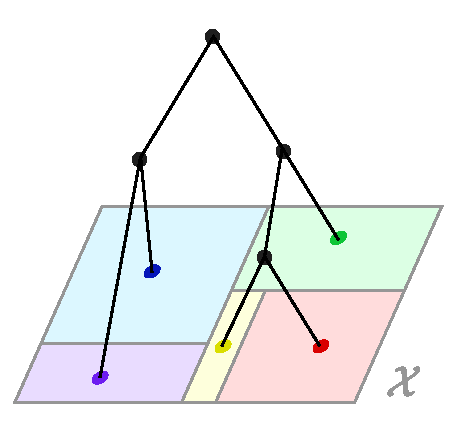
\includegraphics[width=\textwidth]{figma-illustrations/decision-tree}
    \caption{
        Rendering of a decision tree structure. Each inner node corresponds to a partitioning of the parent edge. In standard decision trees, this is a binary partition. In other words, the examples are \textit{split} at a certain value threshold in a certain feature dimension.    }
\end{marginfigure}

\begin{marginfigure}
    \includegraphics[width=\textwidth]{figma-illustrations/tree-partition.pdf}
    \label{fig:tree-partition}
    \caption{A decision tree partitions the data space. For a query example, the corresponding leaf node is determined by traversing the tree downwards from the root node and applying the learned decision criteria.}
% TODO I think this fig does not really provide any value here
\end{marginfigure}


% \marginfigfromsource{fig:decision-tree-boundaries}{symlinks/illustrations/decision-trees/decision-tree-boundaries}
    

There are the following main components to the implementation of a decision tree:
% TODO lowercase "decision tree" always
\begin{itemize}
    \item The \textit{splitting criterion} to apply recursively to subsets of the training data.
    \item The \textit{stopping criterion} that determines whether a node should be split further. This will determine the depth of the decision tree.
    \item The \textit{leaf aggregation function} that produces a prediction for a specific cell. When using the constructed tree for prediction, this will be the leaf node that the query point is assigned to.
\end{itemize}

Like any learner, the quality of a decision tree $q$ is measured with respect to a loss function $\ell$ evaluated over some test set $\{ (x_{i}, y_{i}) \}_{1}^n$. We are ultimately interested in finding a tree that minimises this loss, as an approximate to the generalisation error (see \cref{sec:supervised-learning}).
$$
\frac{1}{n} \sum_{i=1 }^n \ell(y_{i}, q(x_{i}))
$$
% The loss over all examples in a certain leaf (cell) is then 
% $$L(f) \defeq \frac{1}{n_{f}} \sum_{i \in f} \ell(y_{i}, q(f))$$ where $n_{f}$ is the number of points in $f$.

\begin{proposition} $\star$
    \label{thm:decision-trees-impurity}
The choice of loss function, impurity measure and leaf combiner are tightly related and chosing one of these will determine the other choices.
\end{proposition}
The basic idea is that an impurity measure is in fact nothing else than the variance around a centroid. 
If $q(f)$ is chosen to be a centroid with respect to a loss $\ell$, then an impurity measure is exactly the loss of the points in a leaf.

In decision trees, the tree prediction $q$ is constant over a leaf $f$: If $q(f)$ is the output for leaf $f$ then $\forall x \in f: q(x) = q(f)$. Thus, we can write the loss as a sum over the losses of the individual leaves $f$.
\begin{align*}
\frac{1}{n} \sum_{i\in D}  \ell(y_{i}, q(x_{i})) &= \sum_{f \in q} \frac{n_{f}}{n}  
L(f) 
\hspace{1em} \text{for~~ } L(f) \defeq \frac{1}{n_{f}} \sum_{i \in f} \ell(y_{i}, q(f))
\end{align*}
Given a loss function $\ell$ and assuming the tree structure (and thus the leaves $f$) are fixed, how should we define the leaf combiner $q(f)$? From the equation above, we can already see that $L(f)$ is minimised if $q(f) = \arg\min_{z} \sum_{i \in f} \ell(y_{i}, z)$. That is, $q(f)$ is a centroid with respect to $\ell$.
\paragraph{Squared Error and Variance reduction} A commonly used impurity measure for regression is the squared-error variance.
$$
H_{\text{var} }(f) = \frac{1}{n_{f}} \sum_{i\in f} (y_{i} - \bar{y})^2 \hspace{1em} \text{for~} \bar{y} \defeq \frac{1}{n_{f}} \sum_{i \in f} y_{i}
$$
$\bar{y} = \arg\min_{z} \sum_{i \in f} (y_{i} - z)^2$ is a centroid with respect to the squared-error loss.
$q(f) = \bar{y}$ implies $H_\text{var}(f) = L(f)$. In other words, splitting according to $H_{\text{var}}$ minimises the squared-error loss of the tree if the leaf combiner is the arithmetic mean.

\paragraph{\zeroone-loss and majority vote} The majority vote is a centroid with respect to the \zeroone-loss. The implied impurity measure is the error rate.
$$
H_{0/1}(f) = \frac{1}{n_{f}} \sum_{i \in f} \Lzo{y_{i}}{q(f)}
$$

\paragraph{Entropy and Information Gain} We can further express the loss of a leaf $L(f)$ for each of the $k$ classes  separately. Further, let us assume the leaf combiner provides a probability distribution over the classes $k$ (this is without loss of generality since predicting a single class can be seen as a one-hot distribution). Let $q(f)_{k}$ be the $k$-th entry of the distribution $q(f)$. Then
\begin{align}
\begin{split}
\label{eq:leaf-loss-per-class}
L(f) &= \frac{1}{n_{f}} \sum_{i \in f} \ell(y_{i}, q(f)) \\
 % TODO only if loss is "separable"
&= \frac{1}{n_{f}} \sum_{i\in f} \sum_{k} ~\ind{y_{i} = k} ~\ell(k, q(f)_{k}) \\
&= \sum_{k} \sum_{i \in f} \frac{1}{n_{f}} ~\ind{y_{i} = k} ~ \ell(k, q(f)_{k}) \\
&= \sum_{k} p_{fk} ~ \ell(k, q(f)_{k})
\end{split}
\end{align}
where $p_f$ is the class distribution in leaf $f$.
Consider the negative entropy impurity measure
$$
H_{\text{entr} }(f)  = \sum_{k} p_{fk} \log(p_{fk})
$$
If the leaf combiner is the distribution of classes in $f$, i.e. $q(f) = p_{f} = [p_{f_{1}}, \dots, p_{fK}]^\top$ then $H_{\text{entr}}$ maximises $\ell(k, q(x_{i})) = - \log q(x_{i})_{k} = -\log p_{fk}$. Rewriting this over all examples, this is the \textit{log-loss}, also known as \textit{cross-entropy} loss.

\paragraph{Gini impurity} 
To measure the purity of class labels in a cell, one may consider the probability of drawing two different outcomes from the examples in the current cell. 
Let $p_{f}$ be the probability distribution of classes in leaf $f$. Let $p_{fk}$ be the probability of drawing an example of class $k$ from leaf $f$.
The probability of drawing one example of class $k$ and one of a different class is $p_{fk}(1-p_{fk})$.
The probability of drawing two examples of \textit{any} two different classes then is the \textit{Gini impurity}
$$
H_{\text{Gini}}(f) \defeq \sum_{k}p_{fk}(1-p_{fk}) = \sum_k p_{fk} - \sum_k p_{fk}^2 = 1 - \sum_k p_{fk}^2
$$
Analogous to the analysis for $H_{\text{entr}}$, let the leaf combiner be the class distribution in $f$, that is $q(f) \defeq p_{f}$.
From \cref{eq:leaf-loss-per-class}, we can see that $H_{\text{Gini}}$ minimises $\ell(y_{i}, q(x_{i})) = 1 - q(x_{i})_{y_{i}}$, i.e. it maximises the probabilty of the target class.
It remains to be seen that $q(f) = p_{f}$  is in fact a centroid with respect to $\ell$. The centroid is
\begin{align*}
\arg \min_{z} \frac{1}{n_{f}} \sum_{i \in f} (1 - z_{y_{i}}) \equiv \arg\max_{z} \frac{1}{n} \sum_{i \in f} z_{y_{i}}
\end{align*}
Let $e_{k}$ be the vector that contains $1$ at position $k$ and $0$ otherwise. Then 
$$
z_{y_{i}} = \inner{z}{e_{y_{i}}}
$$
Further, $\frac{1}{n_{f}} \sum_{i} e_{y_{i}}$ is exactly the vector of class frequencies $p_{f}$. Continuing, we have
\begin{align*}
\arg\max_{z} \frac{1}{n} \sum_{i \in f} z_{y_{i}} &= \arg \max_{z} \inner{z}{\frac{1}{n} \sum_{i} e_{y_{i}}}  \\
&= \arg \max_{z} \inner{z}{p_{f}}
\end{align*}
which is maximised if and only if $z = p_{f}$.

% We now proceed to define two commonly used splitting criteria. These are the Gini impurity for classification and Variance Reduction (also known as \textsc{Cart}) for regression \cite{tibshirani_ElementsStatisticalLearning_2017}.
% For a splitting function criterion to produce useful decision trees, a reasonable impurity measure should also imply a positive loss gain. Often, this is intuitively clear but particularly for the case of Gini impurity, a comprehensive explanation appears to be hard to find in the literature. We clarify this in the following.




% TODO references for gini impurity and margin maximisation
% - leistner2009 3.1 for def of margin vector, relation to empirical node error
% - sklearn user guide 1.10.7.1 for definition of gini split crit
% - CART
% TODO so, how would this behave if we actually used it for classification? since sqerr sort of reduces to 0-1-loss?


% TODO code snippet illustration plot of margin vector -- should be simple
% TODO disallow page breaks in these boxes
% margin reflects notion of classifier confidence: here, yes, but not necessarily for RF margin


% TODO maybe margin note on tsallis entropies
% TODO cite these two
% information gain and entropy https://stats.stackexchange.com/a/95459/178468
% also note that it doesnt make too much difference: https://stats.stackexchange.com/a/20205/178468


% TODO: i.e. each tree level is sort of a margin boosting step, cf margin analysis of boosting; ADF etc.

% TODO this does not really apply since weve realised traditional DT construction is not so much about breggies... put in outlook where we already mention k-means thing
% \subsubsection{Relationship to $2$-means clustering}
% % TODO different heading that suggests the core statement

% % TODO so "loss gain" / "purity gain" somethign there is really k-means objective?
% % so: decision tree construction = boosting for greedy opt of that? in some sense


% As established in section \ref{sec:splitting-criteria-greedily-minimise-loss-functions}, splitting criteria aim to find a binary partition of the examples in the parent node. The quality of a partition is evaluated according to the purity of the labels. Note that the example features are not considered at all here. If indeed a centroid is chosen as leaf combiner, the notion of impurity is very similar to the objective function of $k$-means clustering on the class labels.
% % TODO this might be a good place to reconsider spaeh


% \subsection{Stopping Criteria \& Tree depth}

% ...


\section{The Random Forest scheme}
\label{sec:random-forest-scheme}

% TODO indeed, high variance of ensemble members is "wanted" in ensembling -- else no room for improvement
% in other words, ensembling only "effective" for high variance learners

The deeper a decision tree is grown, the closer the resultig partition cells will fit the training data. This approximation is in fact guided \textit{only} by the training data. In the extreme case, if the tree is fully grown, each partition cell will correspond to a single example and the outcome of that cell will be the outcome of that example. The tree essentially turns into a $1$-nearest-neighbour scheme with respect to the training dataset. This means that trees constructed with different samples $D$ of training datasets from the original distribution $P(X,Y)$ potentially predict quite different outcomes for testing examples. This is captured in the concept of learner variance as defined in \ref{sec:bias-variance-effects}. 
% In \ref{fig:variance-vs-tree-depth}, one can indeed observe that trees of greater depth have greater variance. At the same time, their fit to the training data improves, which is captured by lower bias.
% TODO maybe reintroduce
% \marginfigfromsource{fig:variance-vs-tree-depth}{symlinks/illustrations/bias-variance/variance-vs-tree-depth}
% so learner variance and correlation are really tightly the same
% \marginnote{
    % TODO extremly randomized trees -> essentially constant variance?
% }

Mitigating this strong dependence on the training data is one of the main motivations of Random Forests. The basic idea is as follows: If we produce several uncorrelated decision trees and average their predictions, then the predictions should exhibit lower variance
In standard forests, this is achieved by introducing randomness into the decision tree construction algorithm by two mechanisms \cite{scornet_ConsistencyRandomForests_2015,breiman_RandomForests_2001}:
\begin{itemize}
\item \textit{Bootstrapping}: Each tree is constructed not on the entire training dataset but a random subset of it. Usually, this \textit{bootstrap sample} is produced by drawing the same amount of points with replacement.
% TODO some considerations on how bootstrapping is actually a vital component
\item \textit{Random feature selection}: When determining where to split a node, not all features are considered but only a random subset of a given size.
% TODO maybe some references....
\end{itemize}

The predictions of individual trees are aggregated to form the forest prediction. Unlike single decision trees, trees in Random Forests are usually grown until each leaf is perfectly pure. Besides their theoretical appeal, Random Forests have several practical advantages.
\begin{itemize}
    \item The construction of individual trees is easily parallelisable.
    \item The trained forest model is relatively small: Only decision rules and leaf outputs need to be stored.
    \item Inference is comparatively fast.
    \item A Random Forest model naturally provides a measure of feature importance \cite{breiman_ClassificationRegressionTrees_2017}.
    \item Random Forests models naturally support classification tasks with more than two target classes.
    \item They are well-suited for problems with extremely high feature dimensionality \cite{yang_ReviewEnsembleMethods_2010}.
    \item There are few hyperparameters to pick and common choices have been shown to work robustly across a wide range of tasks. % TODO cite
    \item They are not prone to overfitting (\cf \cref{sec:diversity-rfs-nns}).
\end{itemize}


\subsection{Bagging}
\label{sec:bagging}

\marginnote{
In uniform bootstrapping, if we draw $n$ samples from $n$ available points, the probability of an example being selected in a single draw is $\frac{1}{n}$. Conversely, the probability of an example not being selected in a single draw is $1-\frac{1}{n}$. We draw $n$ times. Hence, the probability of an observation not being selected in any of the draws is $(1-\frac{1}{n})^n$. The probability of an example indeed being selected in at least one of the draws then is $1 - (1 - \frac{1}{n})^n$.  For large $n$, one can approximate $\lim_{ n \to \infty }1-(1-\frac{1}{n})^n = 1- e^{-1} \approx 0.632$ \cite{buschjager_ThereNoDoubleDescent_2021}.
}
A vital ingredient to Random Forests is the \textit{Bagging} procedure, which stands for \textit{bootstrapping and aggregating}. Bagging is an ensemble learning technique not specific to Random Forests. In Bagging, each member is constructed not on the full training dataset but a \textit{bootstrap sample} of it. The bootstrap sample is usually determined by drawing $n$ out of $n$ examples uniformly with replacement \cite{breiman_RandomForests_2001,buschjager_GeneralizedNegativeCorrelation_2020}. We will refer to this as \textit{uniform bootstrapping}. One can also determine the bootstrap sample by drawing $n$ out of $n$ points with replacement according to a probability distribution $\{p_1, ..., p_n\}$, which we call \textit{weighted bootstrapping}. Bootstrapping means that each member is trained on a different dataset. 


% randomization

% \subsection{Random Forests converge}


% As the number of trees increases, for almost surely all sequences $(\Theta_{1}, \dots)$, the generalisation error $PE^\star$ converges:
% $$
% % TODO uhh doesnt really make sense, check reference
% \mathbb{E}_{(X,Y), D}\left[ \ell(Y, q_{D}(X)) \right]  \to
% % PE^\star \to 
% % \prob{\vec{X}, Y}{\left(\prob{\Theta}{q(\vec{X}, \Theta)=Y} - \max_{j \neq Y} \prob{\Theta}{q(X; \Theta) = j } \right) < 0
% % } = 
% \prob{\vec{X}, Y}{
% \mr(\vec{X}, Y)  < 0
% }
% $$

\subsection{Tree and Forest Partitions}
\label{sec:tree-and-forest-partitions}

The generalisation error, and consequently individual terms of any decomposition of it have been defined point-wise. That is, they are measured by an expectation over possible realisations of example-outcome pairs $(X,Y)$. They further depend on a random variable $D$ representing the training input to the learner. In order to estimate such an expectation for a given model (a realisation of $D$), one has to sample realisations of $(X,Y)$. In practise, these example-outcome pairs typically come from a validation dataset that was withheld from training.
We have seen in \cref{sec:diversity} that for some losses, diversity can be expressed independently of the outcome variable $Y$. 
To approximate an actual value, we would still need to sample realisations of $X$.

Decision Trees, particularly if grown deeply, can be considered to \textit{approximate} the training data, i.e. they are a lossy representation of the training data. A grown decision tree model contains two kinds of parameters, both derived from the training data $D$.
\begin{itemize}
\item The tree structure, i.e. the decision boundaries. These are used for determining the leaf node for a query example.
\item The output value of a leaf node. This is the predicted value for a query example falling into that leaf. The leaf predictions depend on the decision boundaries but are not solely determined by them. 
\end{itemize}
% TODO plot of approximated polynomial
This leads to the question whether characteristics of a Random Forest model could be expressed solely in terms of its tree parameters, and not in terms of predictions on query points.
% In the case of a forest of trees, one would expect that if the trees have different decision boundaries, the forest is more diverse. 
% Further, this would provide a way to express diversity \textit{in terms of model parameters} and not in terms of predictions on query points.
% In the case of a forest of trees, one would expect that if the trees have different decision boundaries, the forest is more diverse. 

\begin{marginfigure}
    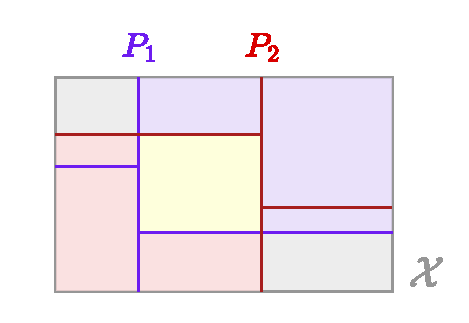
\includegraphics[width=\textwidth]{figma-illustrations/forest-partition.pdf}
    \label{fig:forest-partition}
    \caption{The \tcircle{gray} data space $\mathcal{X}$ (gray) and partitions \tcircle{purple} $P_1$ and \tcircle{red} $P_2$  of it induced by two decision trees. The \tcircle{yellow} intersections of any cell of $P_1$ and any cell of $P_2$ form the \textit{forest partition}. One such intersection is highlighted in yellow.
    }
\end{marginfigure}
Each level of a decision tree induces a partition of the space of examples $\mathcal{X}$. Because each example is associated with an outcome, we can also think of it as a partition of $(\mathcal{X}, \mathcal{Y})$. We call such a partition a \textit{tree partition} and a cell a \textit{tree cell}.
Decision trees produce predictions via an aggregate of the queried leaf node's outcomes. Thus, the predictions of a decision tree over a single cell are constant.
An ensemble of trees also induces a partition: the partition obtained by intersecting all tree partitions. We call these \textit{forest cells}. Formally, if $T_{1}, \dots, T_{M}$ are tree partitions, the forest partition is given as
$$
\{ c_{1} \cap \dots \cap c_{M} ~|~ c_{1} \in T_{1}, \dots, c_{M} \in T_{M}\}
$$
Each forest cell is associated with $M$ tree cells whose intersection constitutes it.
For any query point that falls within a certain tree cell, the forest prediction is given by an aggregate over the associated tree cells. Thus, the predictions of a random forest are constant over a single forest cell.
This means that also a loss, as well as any decomposition constituents of the loss are constant over forest cells.

Exploiting that partitions are cell-wise constant, we can apply a special case of the law of total expectation to express it in terms of cells.
\sidenote{
% TODO move to lemma in prelims
Let $X_{1} \dot\cup \dots \dot\cup X_{M}$ be a disjoint, countable partition of the sample space of $X$. Then
$$
\mathbb{E}_{X}\left[ X \right] = \sum_{i=1}^M  \mathbb{E}_{X}\left[ X ~|~X_{i} \right] \cdot \prob{}{X_{i}}
$$
}
Consider a forest partition $Z = Z_{1} \dot\cup \dots \dot\cup Z_{P}$ of $Z=(X,Y)$. 
\begin{proposition} 
   \label{thm:random-forest-structure} 
    $\star$ The generalisation error of a random forest model can be expressed in terms of intersections of tree cells.
% TODO definitions
$$
\mathbb{E}_{Z,D}\left[ \ell(y,\bar{q}) \right] = \mathbb{E}_{Y,D}\left[ \sum_{p=1}^P \prob{}{Z_{p}} \cdot \mathbb{E}_{Z}\left[ \ell(Y, \bar{q}) ~|~Z_{p}\right]   \right] 
$$
\end{proposition} 
% TODO maybe more precise derivation
A similar statement can be made for the simpler case of a single decision tree and is used in \cref{sec:decision-trees} to derive impurity measures.

While we have eliminated the dependence on a query point $X$, the quantity $\mathbb{E}_{Z}\left[ \ell(y, \bar{q}) ~|~Z_{p}\right]$ still depends on a realisation of an outcome $Y$. In \cref{sec:diversity-rfs-nns} we see that we can decompose this term further into components that are dependent and independent of $Y$, respectively.


\end{document}